\documentclass[12pt, twoside]{article}
\usepackage[francais]{babel}
\usepackage[T1]{fontenc}
\usepackage[latin1]{inputenc}
\usepackage[left=7mm, right=7mm, top=5mm, bottom=5mm]{geometry}
\usepackage{float}
\usepackage{graphicx}
\usepackage{array}
\usepackage{multirow}
\usepackage{amsmath,amssymb,mathrsfs} 
\usepackage{soul}
\usepackage{textcomp}
\usepackage{eurosym}
 \usepackage{variations}
\usepackage{tabvar}

\begin{document}

\section*{\center{Correction devoir surveill� 6}}


\subsection*{Exercice 3}

\begin{enumerate}
\item Le potager est un triangle rectangle dont on conna�t deux c�t�s. D'apr�s
le th�or�me de Pythagore, on peut calculer le troisi�me c�t�.
\item Le triangle ABC est rectangle en A. D'apr�s le th�or�me de Pythagore, on
a:

\enskip

$BC^2=AC^2+AB^2$

$10,59^2=AC^2+6,75^2$

$112,1481=AC^2+45,5625$

$AC^2=112,1481 - 45,5625 = 66,5856$

\enskip

La longueur AC est positive donc AC=$\sqrt{66,5856}=8,16$ m. 

On peut maintenant calculer la longueur qu'il faut pour la cl�ture: 8,16 +
10,59 + 6,75 = 25,5 m.
\end{enumerate}


\subsection*{Exercice 4}

\begin{tabular}{cc}
\begin{minipage}{10cm}
\begin{enumerate}
  \item [2.] Le triangle ABO est rectangle en O. D'apr�s le th�or�me de
  Pythagore, on a:


$AB^2=AO^2+OB^2$

$AB^2=3^2+6^2$

$AB^2=9+36$

$AB^2=45$


 
 
 On a bien  $AB^2=45$.
 \end{enumerate}
\end{minipage}
&
\begin{minipage}{8cm}
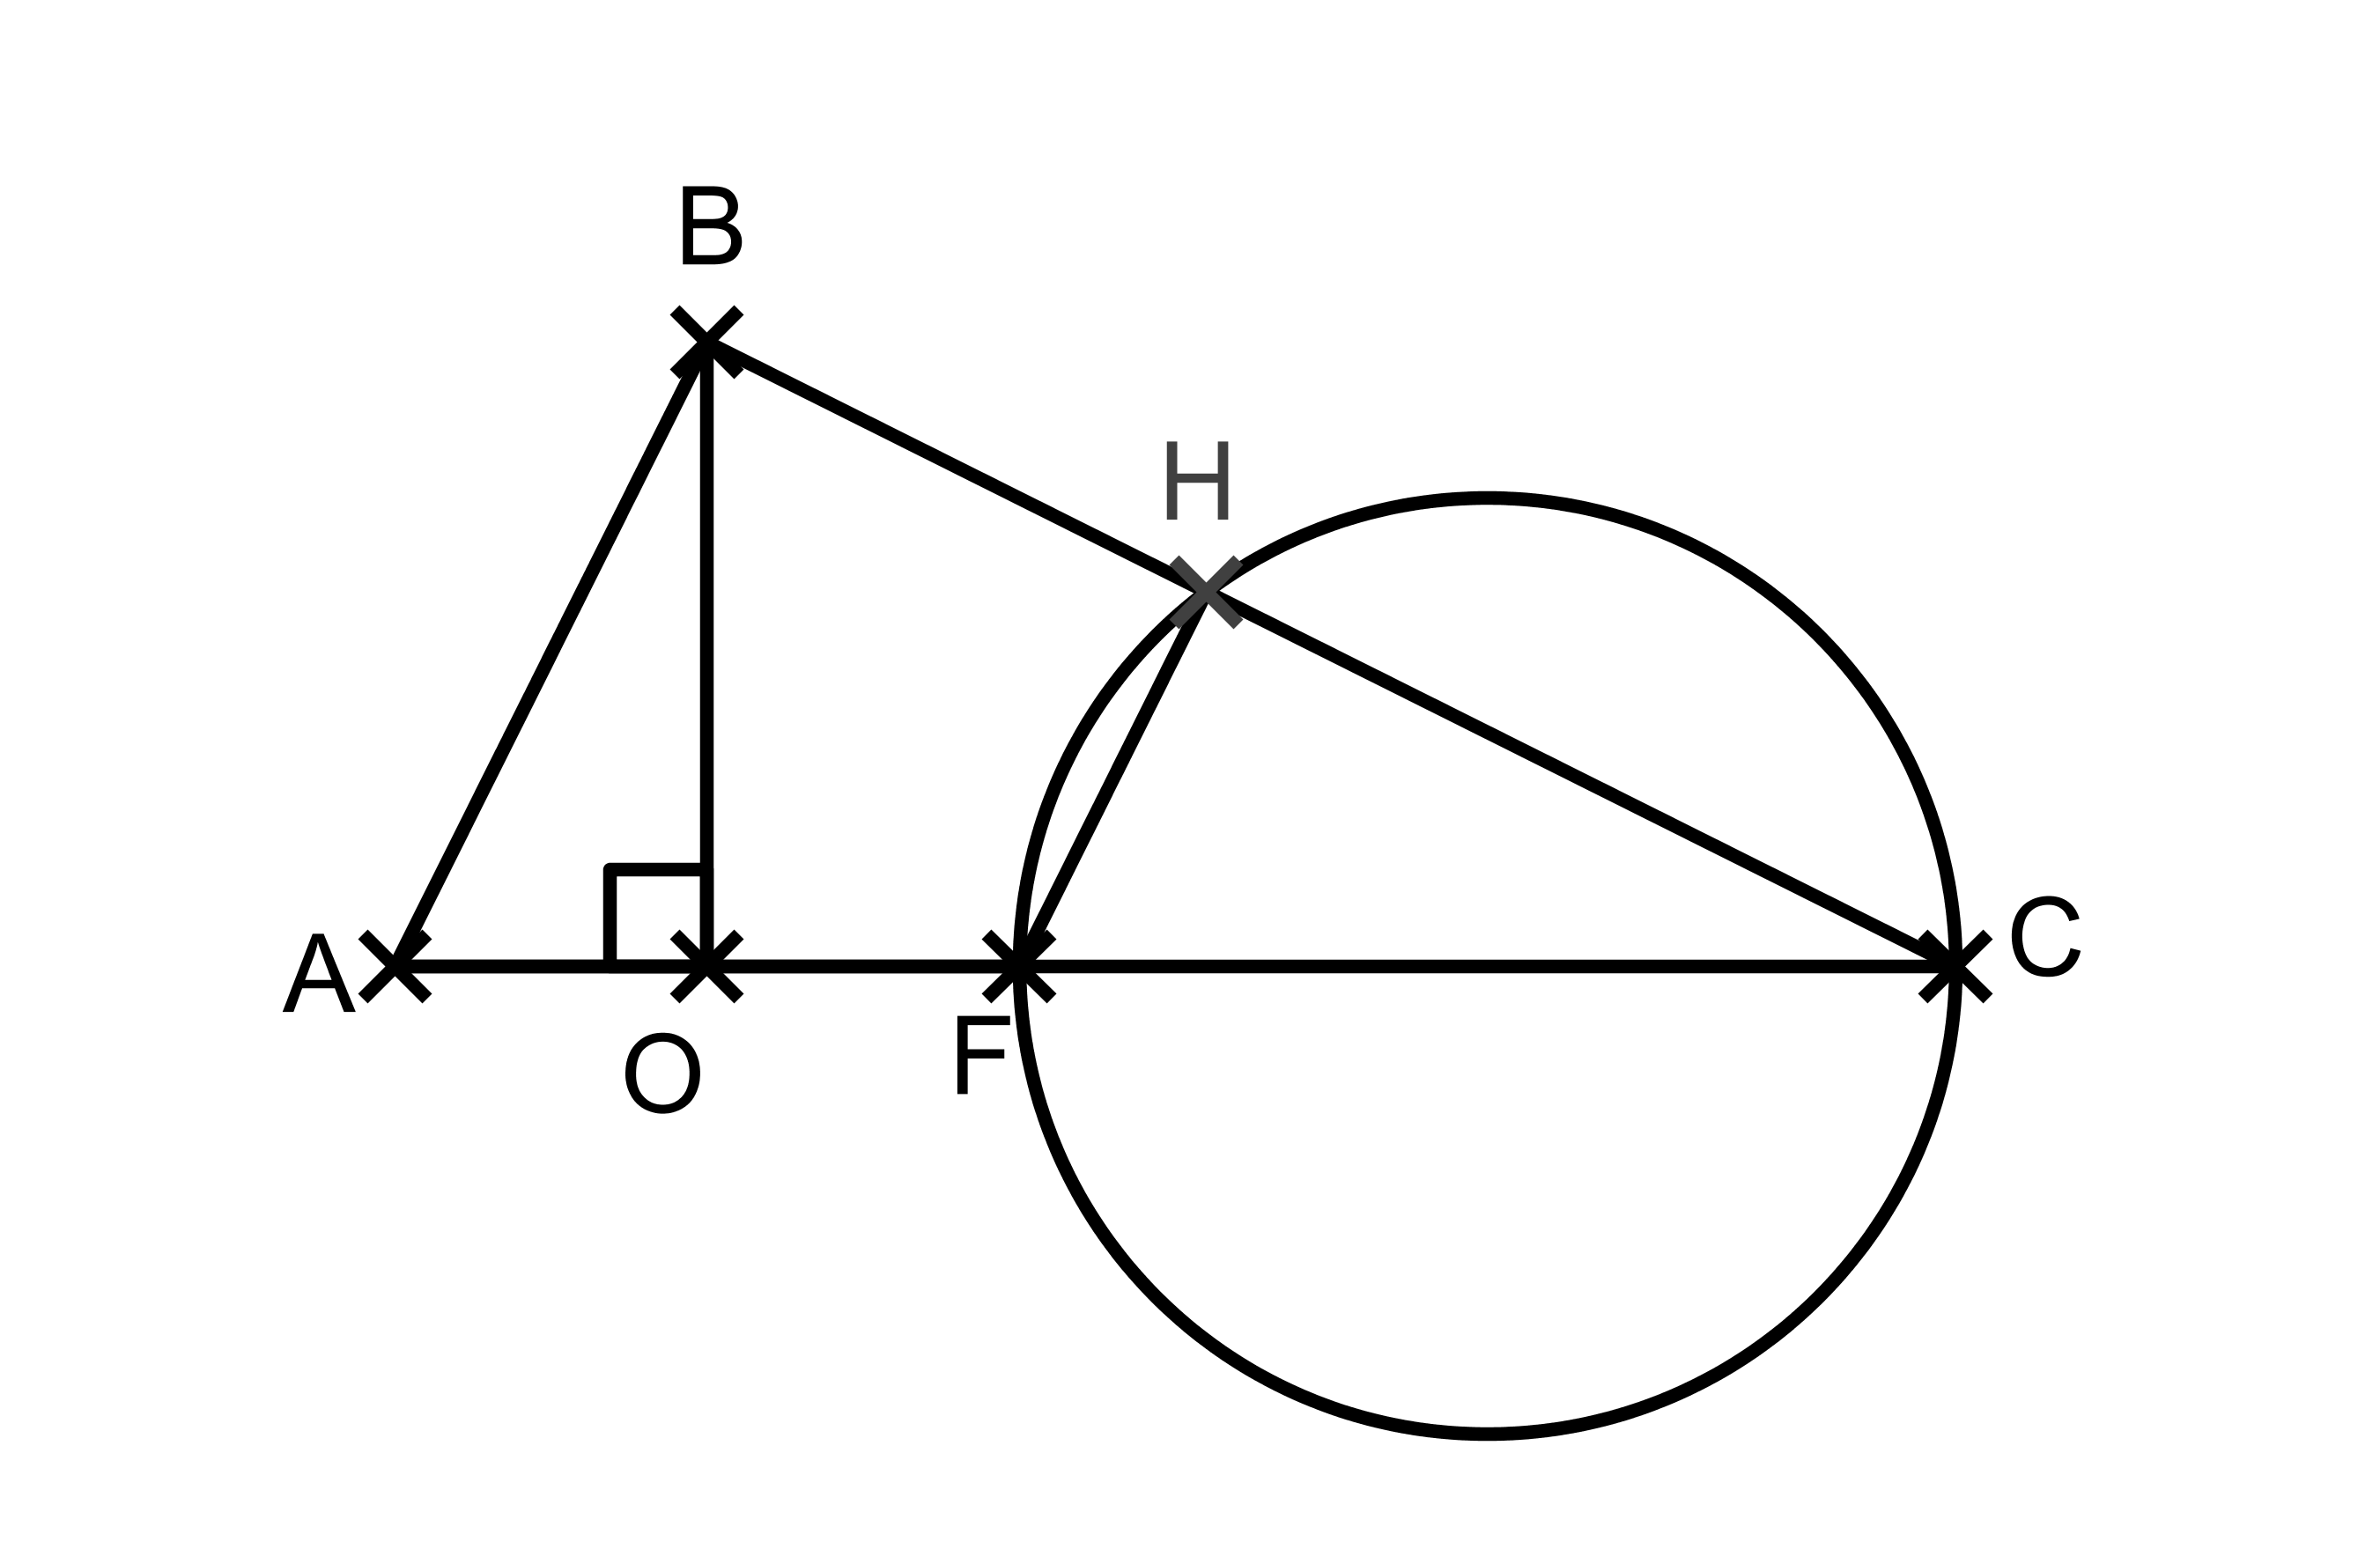
\includegraphics[width=6cm]{images/ex4.png}
\end{minipage}
\end{tabular}


\begin{enumerate}
 \item [3.] OC= 15 - 3 = 12 cm. Le triangle OBC est rectangle en O. D'apr�s le
 th�or�me de Pythagore, on a:
  

$CB^2=CO^2+OB^2$

$CB^2=12^2+6^2$

$CB^2=144+36$

$CB^2=180$

 
 
 On a bien  $CB^2=180$.  



\item [4.] Dans le triangle ABC, le plus long c�t� est [AC]. Donc on calcule s�par�ment
$AC^2$ et $AB^2+BC^2$. D'apr�s les questions pr�c�dentes, on sait que
$CB^2=180$ et $AB^2=45$.

\enskip

\begin{tabular}{cc}
\begin{minipage}{8cm}
\begin{tabular}{c|c}
$AC^2=15^2$  &  $AB^2+BC^2=45+180$ \\
$AC^2=225$  &  $AB^2+BC^2=225$\\
 
\end{tabular}
\end{minipage}
&
\begin{minipage}{9cm}

On constate que  $AC^2 = AB^2+BC^2$. D'apr�s la r�ciproque du th�or�me de
Pythagore, le triangle ABC est rectangle en B. Donc les droites (AB) et (BC)
sont perpendiculaires.
\end{minipage}
\end{tabular}




\enskip

\item[6.] Le triangle FHC est inscrit dans le cercle de diam�tre [FC]. D'apr�s
la propri�t� ``si un triangle est inscrit dans un cercle de diam�tre l'un de ses
c�t�s alors ce triangle est rectangle et admet ce c�t� pour hypot�nuse'', on en
conclut que le triangle FHC est rectangle en H.

\enskip


\item[7.] Les droites (AB)et (FH) sont toutes les deux perpendiculaires � la
droite (BC). D'apr�s la propri�t� ``si deux droites sont perpendiculaires � la
m�me droite alors elles sont parall�les entre elles'', on en d�duit que les
droites (AB) et (FC) sont parall�les.

\end{enumerate}
\end{document}
